\documentclass{proc}
\usepackage{graphicx}
\graphicspath{ {./images/} }

\begin{document}
	
	\title{Perceptually-Optimized Animations for Correlation Judgment and Visualization}

	
	\author{Truman Larson, Lane Harrison}
	
	\maketitle
	
	\section{Introduction}
		Animation provides a unique opportunity to reinforce perceptual ideas pertaining correlation judgment. Yang suggests that people use "visual features" when judging correlations \cite{Yang2019}. However, the aspects of perception considered here are purely static. 
		
		We are proposing an expansion of considered visual features to include animated visualizations as a potential method for perception. Mental translation has been found to be a factor for matching patterns between objects and would be a candidate for a visual task people perform \cite{larsen1998effects}. Others tasks may include mental rotation or some other form of visual imagery. 
		
		Following similar methodologies of past experiments like Yang, such as Harrison et al \cite{Harrison2014}, we will be testing to see whether the inclusion of these animation has an effect on participant performance. If animated feedback on the judgments differs from similar non-animated methods, our results will demonstrate that people may use some sort of visual translation or rotation task to process these comparisons.
	\section{One-sentence description}
		Expanding upon previous idea of correlation judgment, we are applying animation to determine if people utilize mental translation or rotation when judging correlation. 
	\section{Project Type}
		Experiment (crowd-sourced)
	\section{Audience} 
	\begin{quote}
		\textit{Who is the audience for this project? 
			How does it meet their needs? 
			What happens if their needs remain unmet?}
	\end{quote}
		Animation has been researched as a way to make presentations more interesting and engaging \cite{Robertson2008}. The core reasons why animation can be effective deserve exploring. Within correlation judgment, there are many opportunities to understand how people make these judgments with the work done by Yang \cite{Yang2019}. Expanding this research to include animation can give a concrete basis for its usage within visualization of many kinds. 
		If animation continues to be under-researched, it will remain a missed opportunity for many different areas of visualization.  
	\section{Approach}
		\begin{figure}[t]
			\centering
				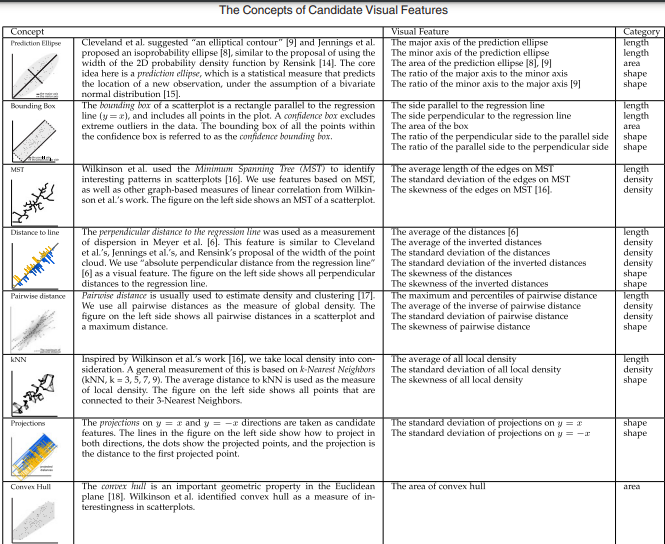
\includegraphics[width=0.5\textwidth]{concepts}
				\caption{List of conceptual visual features Yang theorized for how we perceive correlation in scatterplots.}
			\label{fig:concepts}
		\end{figure}
		Expanding of the above list of ideas used in Yang, we will add animation in the form of translation and/or rotation to most of these methods \cite{Yang2019}. We will utilize the same method of evaluation as Yang to determine the specific animated features preform the best. The experiement method is outlined below.
		\begin{figure} [t]
			\centering
				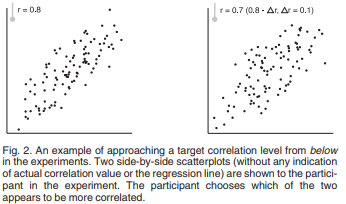
\includegraphics[width=0.5\textwidth]{methods}
				\caption{Methods used by Yang}
			\label{fig:methods}
		\end{figure}
		We will use this method in the way outlined by Yang in order to directly be able to compare our results

	\subsection{Evidence for Success}
	\begin{quote}
		\textit{Why do you think it will work?} 
	\end{quote}
		Based off the research done by Rensink \cite{Rensink2017} and Yang \cite{Yang2019}, there is a basis for evaluating judgment of correlation. Animation is just another dimension added on to this research that has the potential to capture other human perception ideas outlined in \cite{larsen1998effects}. 
	
	\section{Best-case Impact Statement}
	\begin{quote}
		\textit{In the best-case scenario, what would be the impact statement (conclusion statement) for this project? }
	\end{quote}
		In the best case, we will see similar results to Yang and Rensink. Additionally, we will see that animation as a feature has an effect on user performance. Ideally, this research will lay the groundwork for how animation effects human perception and give scientific basis for the inclusion of animation for a perceptual psychology standpoint. 
		If this succeeds, further research can explore exactly which animations provide the optimal increase in understanding. 
	\section{Major Milestones}
	\begin{itemize}
		\item Replicate Yang's design
		\item Determine what additional feedback to include from the concepts: ellipse, box, KNN, etc
		\item Determine exact animations to use
		\item Pilot the design with all animations and feedback
		\item Full experiment to compare animation vs no animation (not in scope of class)
	\end{itemize}
	\section{Obstacles}
	
	\subsection{Major obstacles} % (if these fail, the project is over)
	\begin{itemize}
		\item Some of the visual concepts are difficult/time consuming to replicate. To get a wide range of these will require great investment that may be out of scope.
		\item Most participants may not know to use the feedback. This feedback might not achieve anything if people don't already use some form of mental translation.
	\end{itemize}
	\subsection{Minor obstacles}
	\begin{itemize}
		\item Much of the design may have to be adapted from existing code/resources. Integrating many different experiments may cause issues. 
		\item Getting a full experiment out takes finacial resources and additional time and thus might not be in scope for the project, but rather an entire research project on its own. 
	\end{itemize}
	\section{Resources Needed}
	\begin{quote}
		\textit{What additional resources do you need to complete this project?}
	\end{quote}
	\begin{itemize}
		\item Code and additional setup for the experiment
		\item Code and algorithms for the visual features
		\item Additional resources on perceptual psychology to inform the animation design
		\item Financial resources and additional time to complete a full experiment. 
	\end{itemize}
	\section{5 Related Publications}
	\begin{quote}
		\textit{List 5 major publications that are most relevant to this project, and how they are related}
	\end{quote}
	\begin{itemize}
		\item Yang provided the idea of visual features and a list of potential ones \cite{Yang2019}.
		\item Rensink created systems to evaluate the results of correlation judgment experiments \cite{Rensink2017}.
		\item Robertson evaluated the current status of animation use in animation and provided alternatives and criticisms \cite{Robertson2008}.
		\item Larsen developed methods to understand visual perception and mental translation \cite{larsen1998effects}.
		\item Li was able to compare performance for very different methods of visualizing correlation, which could be useful to apply between animated and static feedback \cite{Li2010}.
	\end{itemize}
	\section{Define Success}
	\begin{quote}
		\textit{What is the minimum amount of work necessary for this work be publishable?}
	\end{quote}
	To publish a full paper, ideally an controlled experiment with animated vs non-animated feedback would be conducted. Anything that has the potential to show the difference could be publish. In the context of this class, however, a pilot study with ~10 participants may be more suitable to get an idea for how viable an experiment like this is. 
	\bibliographystyle{abbrv}
	\bibliography{prospectus}
\end{document}